% Copyright (c) 2014,2016 Casper Ti. Vector
\chapter{系統設計}

\section{區塊鏈的實名交易監督系統設計}

	本論文提出區塊鏈的實名交易監督系統(Blockchain Real-name Transaction Monitoring System,BRTMS),以下簡稱BRTMS,BRTMS以加密貨幣比特幣實作,BRTMS包含三個子系統,商店和商品信息管理子系統(Store and Merchandise Information Management Sub-System,SMIMSS)、商家移動裝置收款及交易子系統(Store Mobile payment Collection and Transaction、Sub-System,SMCTSS)、客戶端移動支付和交易子系統(Client Mobile Payment and Transaction Sub-System,CMPTSS),圖\ref{model0}為主系統與子系統的功能模塊圖。


	\begin{figure}[!htbp]
		\centering
		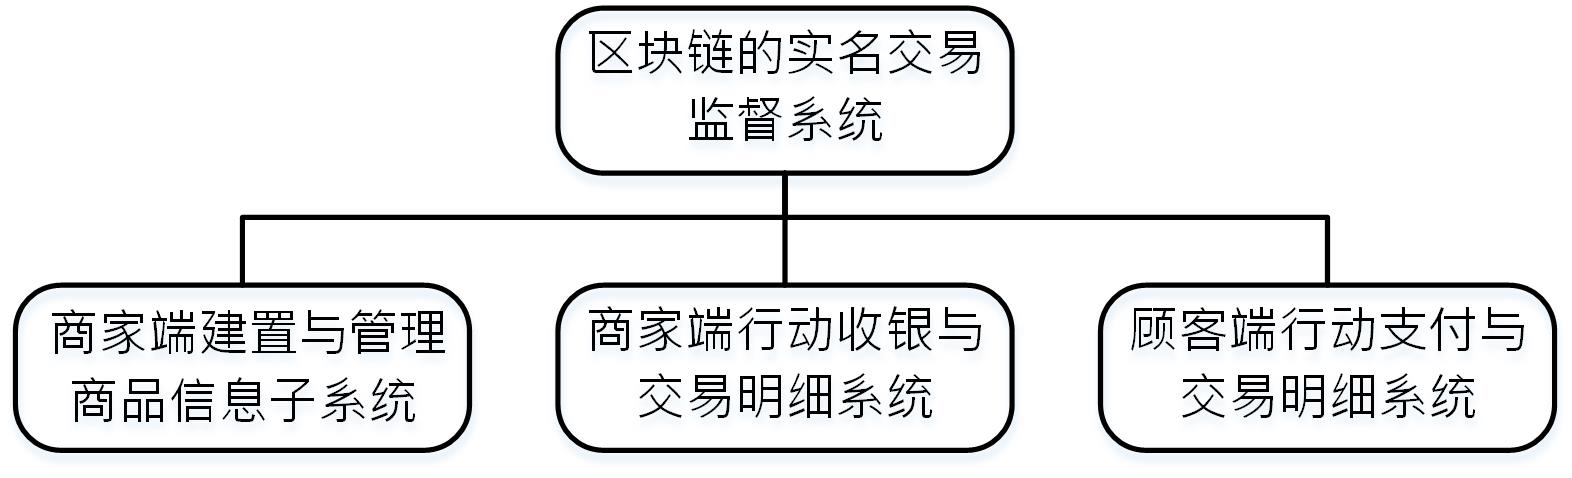
\includegraphics[width = 0.8\textwidth]{model0.jpg}
		\caption{BRTMS系統功能模塊圖}\label{model0}
	\end{figure}

	本論文將開發讓商家能夠結合商品與RFID標籤,以達到快速建構與管理商品資料庫之系統,並且讓商家及顧客可以運用手機NFC功能來實際運作比特幣的行動支付流程。店家只需要掃描商品上的RFID標籤,即可快速建立交易清單,再利用NFC功能與顧客之行動裝置進行訊息交換,輕鬆地將商家的收款地址以及交易資料傳送給顧客,收到資料後便能快速地以顧客之比特幣行動電子錢包付款,並將交易細項儲存下來,以便未來商家與顧客能夠快速查詢比特幣行動支付的交易紀錄。
	本系統主要是以完成區塊鏈之數位加密貨幣的收款監督系統為主要目標,本論文進而將積極利用自由軟體的利基:使用成本低、進入門檻低、開放原始碼、社群能力強、共通性及移植性強、資通安全性高等優勢來開發本論文收款監督系統的應用服務平台。本系統範圍包含建置下面主系統與各項子系統如下:
		\begin{enumerate}
		\item 區塊鏈的實名交易監督系統(Blockchain Real-name Transaction Monitoring System, BRTMS)
		\item 商家端建置與管理商品資訊子系統(Store and Merchandise Information Management Sub-System,SMIMSS):本系統可以讓商家在進貨時,快速地將RFID標籤之識別碼與進貨商品資訊集成在一起,並且透過本系統新增、修改或刪除資料庫內部的資訊,包括產品名稱、詳細資訊,存貨數量等資訊,商家與顧客便可依照該資料庫取得當前商品資訊與狀態。不僅讓商店的存貨資訊更加清楚明瞭,也可以提供顧客更多的即時服務,圖\ref{model1}所示。

			\begin{figure}[htbp]
			\centering
			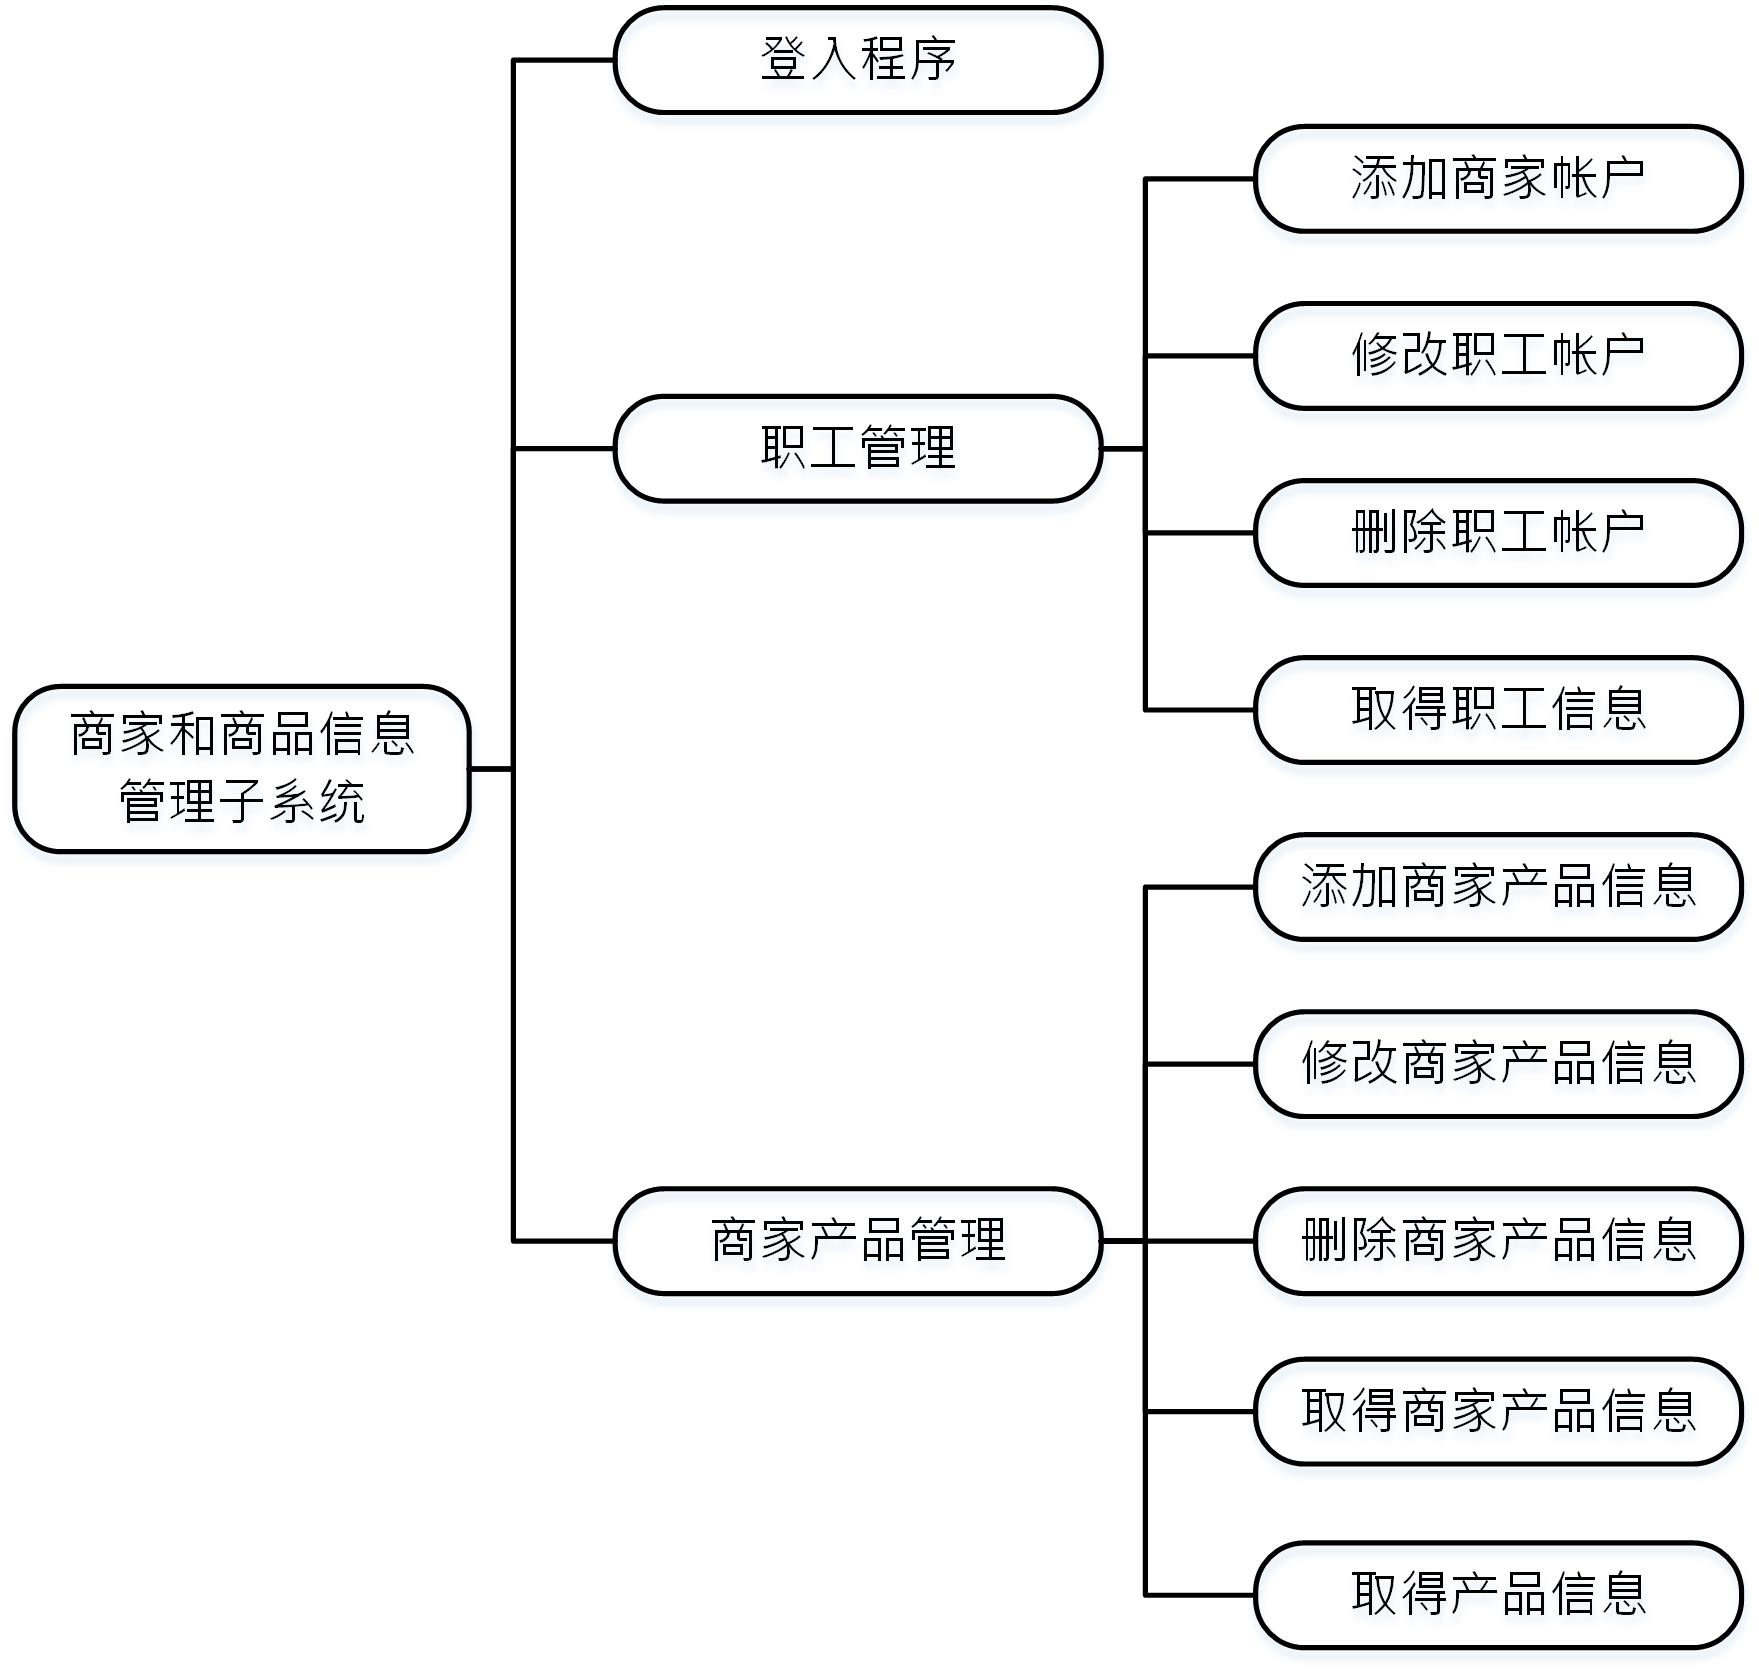
\includegraphics[width = 0.8\textwidth]{model1.jpg}
			\caption{商家端建置與管理商品資訊子系統功能模塊圖}\label{model1}
			\end{figure}



		\item 商家端行動收銀與交易明細系統(Store Mobile payment Collection and Transaction Sub-System,SMCTSS):本系統使商家在結帳時,能夠以手機NFC功能掃描商品上的RFID 標籤,即可簡單地建立交易清單,並透過NFC與顧客手機碰觸,將交易清單以及商家之比特幣收款地址等等重要交易資訊一併傳遞給顧客,可以簡短結帳的速度,使結帳效率大幅提升,圖\ref{model2}所示。
		 
			\begin{figure}[htbp]
			\centering
			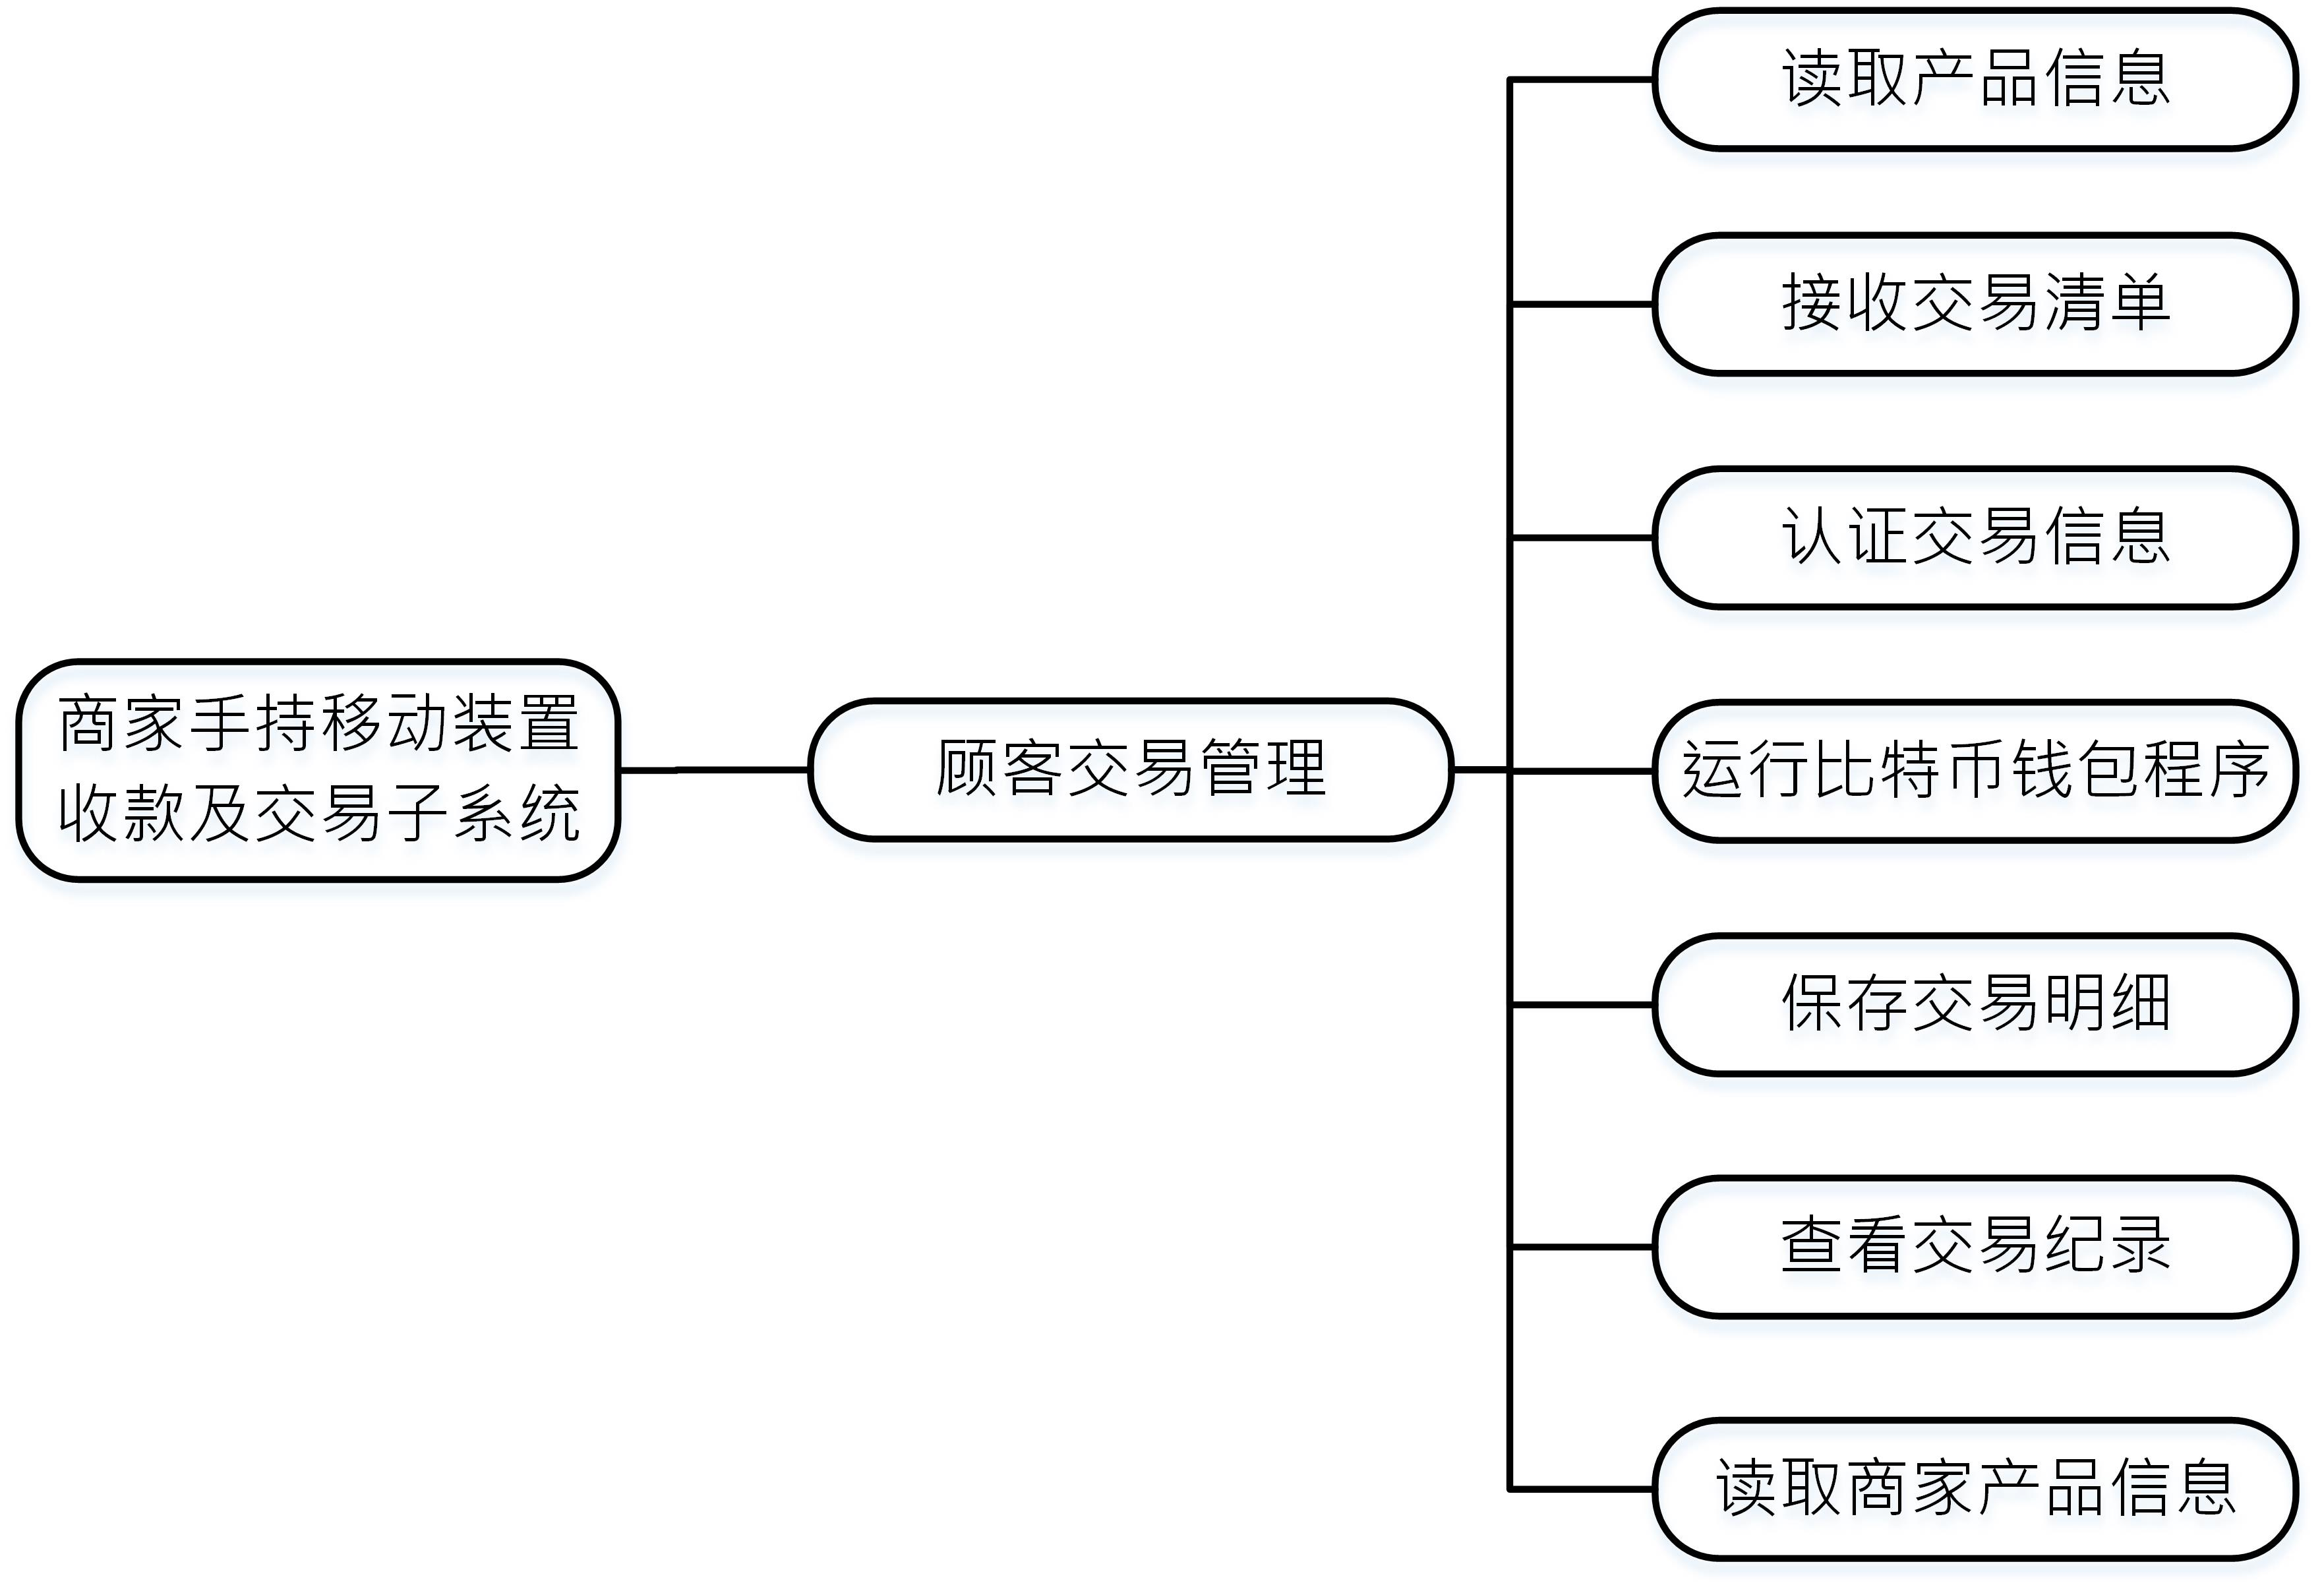
\includegraphics[width = 0.8\textwidth]{model2.jpg}
			\caption{商家端行動收銀與交易明細系統功能模塊圖}\label{model2}
			\end{figure}


		\item 顧客端行動支付與交易明細系統(Client Mobile Payment and Transaction Sub-System,CMPTSS):顧客在結帳時,不必再麻煩的拿出信用卡或是零錢包,只需要拿出手機讓店員以NFC將交易清單與比特幣地址轉送給自己,即可自動連結至比特幣電子錢包的應用程式當中,並且自動填妥相關資料,如:交易金額、收款地址等等與此同時也能將交易紀錄儲存於客戶端,以便日後顧客快速取得過往的交易紀錄,除此之外亦可讓廣大的民眾體驗數位加密貨幣與行動支付帶來的便利生活。
			\begin{figure}[htbp]
			\centering
			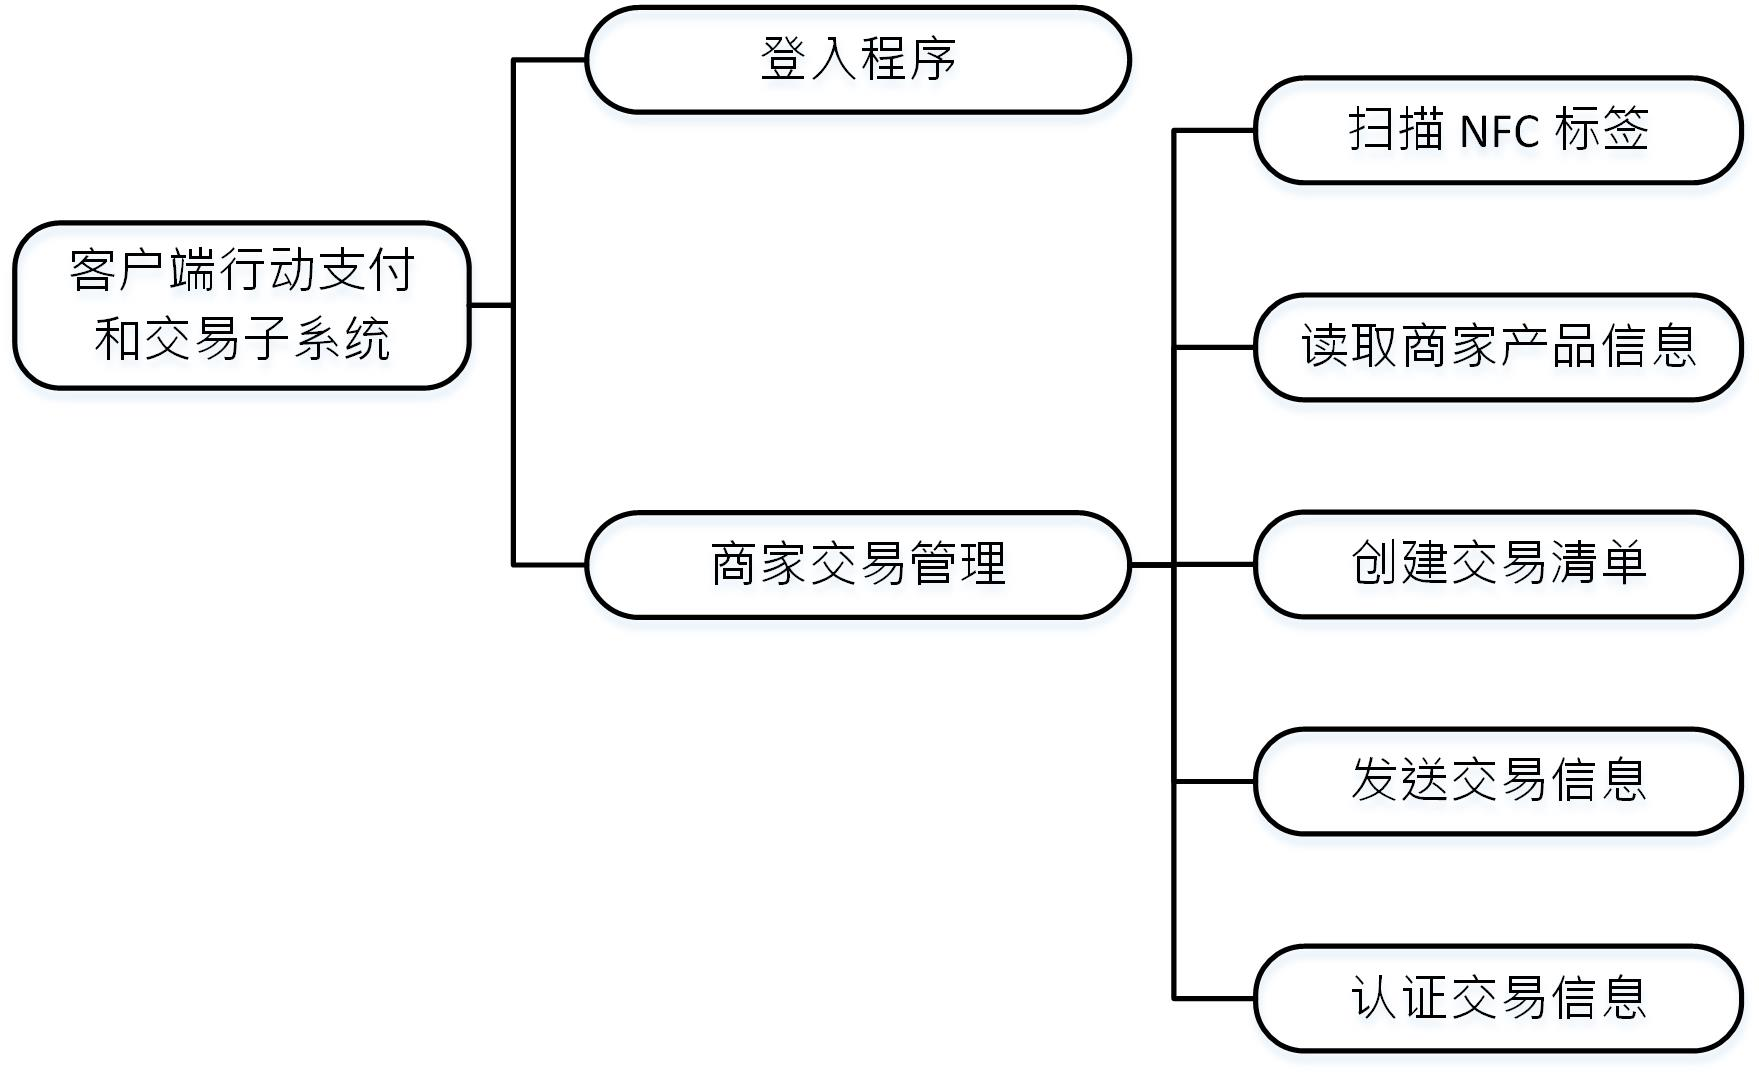
\includegraphics[width = 0.8\textwidth]{model3.jpg}
			\caption{顧客端行動支付與交易明細系統功能模塊圖}\label{model3}
			\end{figure}
		
	\end{enumerate}
	\subsection{BRTMS數據庫設計}

	區塊鏈的實名交易監督系統應用了六個信息表,分別為商家信息、產品信息、交易信息、用戶信息、職工信息以及商家產品信息,以下將逐一說明:

		\begin{figure}[htbp]
			\centering
			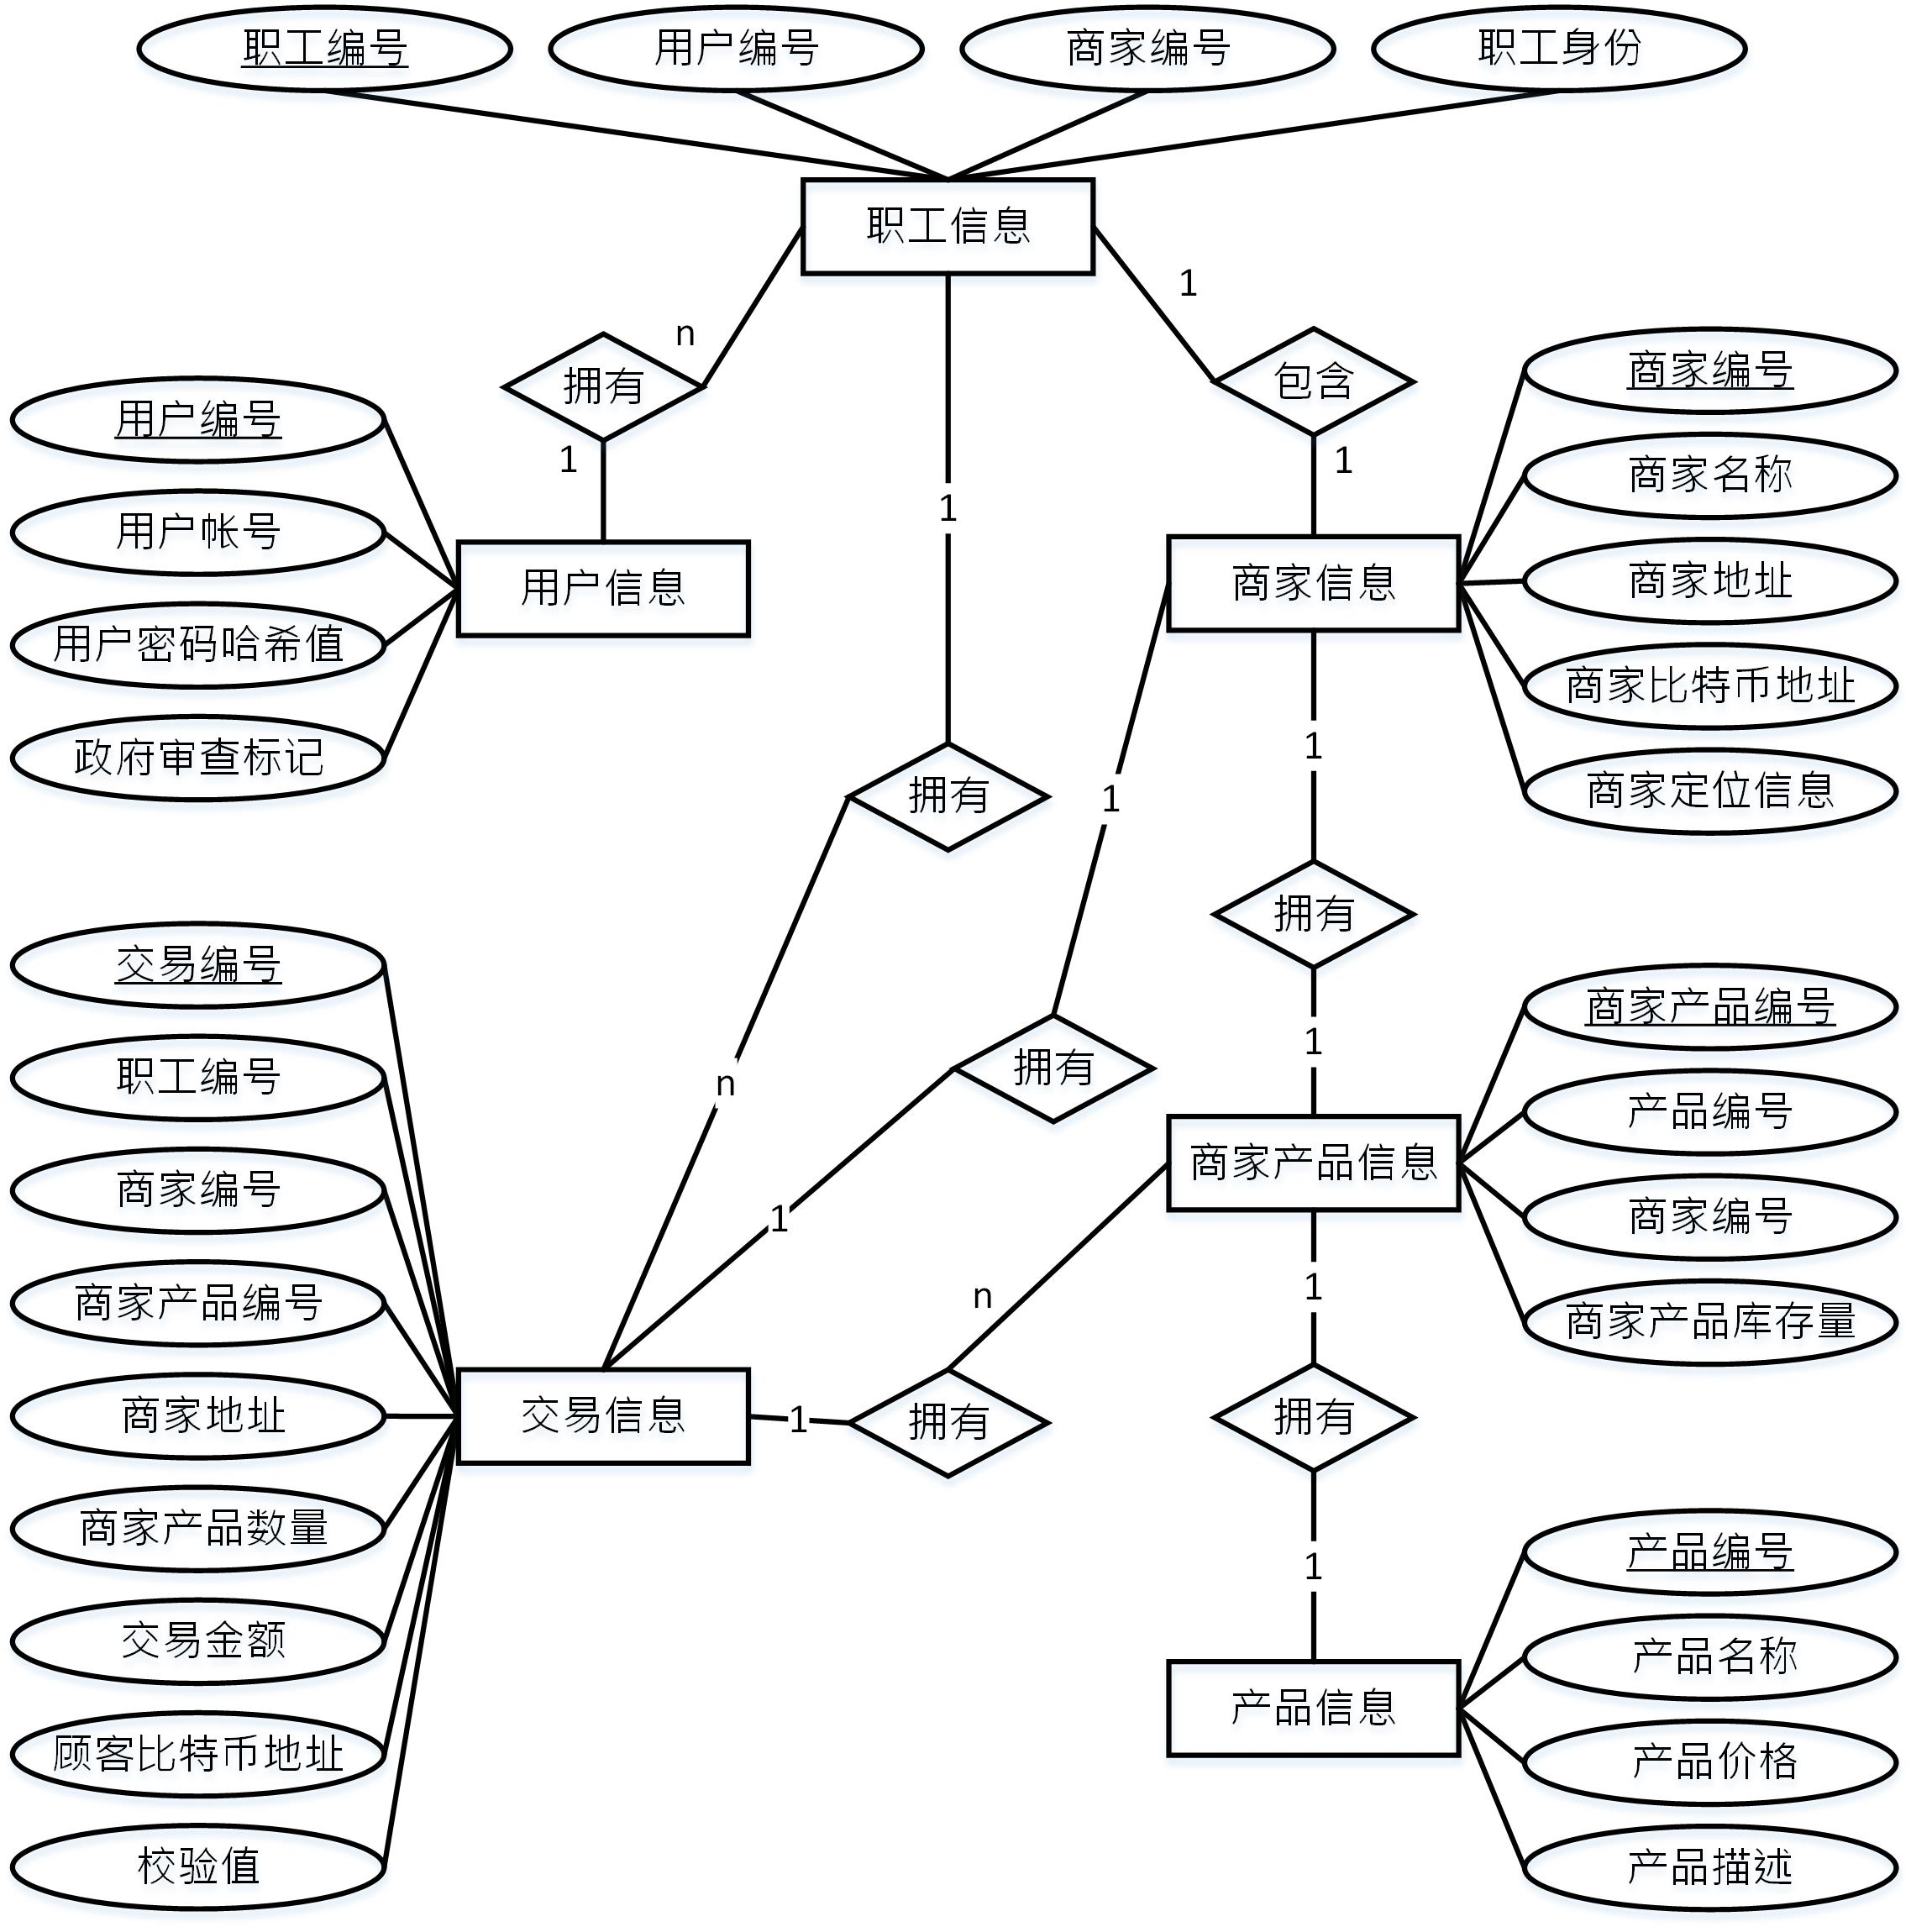
\includegraphics[width = 1\textwidth]{er.jpg}
			\caption{BRTMS數據庫實體關係圖}\label{db}
		\end{figure}

		\begin{enumerate}
		\item 商家信息表:存儲正在審核中的企業信息或已經過審核的企業信息。表\ref{store}存儲的信息包括商家編號、商家名稱、商家地址、商家比特幣地址以及商家定位信息。


				\begin{table}[!htbp]
				\centering
				\caption{商家信息表}
				\label{store}
				\resizebox{\textwidth}{!}{%
				\begin{tabular}{|c|c|c|c|c|c|}
				\hline
				序號 & 字段名 & 字段說明 & 類型 & 是否為空 & 主外鍵 \\ \hline
				1 & STORE\_ID & 商家編號 & int & 否 & PK \\ \hline
				2 & STORE\_NAME & 商家名稱 & navarchar(20) & 否 &  \\ \hline
				3 & STORE\_ADDRESS & 商家地址 & navarchar(50) & 否 &  \\ \hline
				4 & STORE\_BTCADDRESS & 商家比特幣地址 & navarchar(50) & 否 &  \\ \hline
				5 & STORE\_GPS & 商家定位信息 & navarchar(30) & 否 &  \\ \hline
				\end{tabular}%
				}
				\end{table}

		\item 產品信息表:只有授權用戶才能登錄添加或修改交易產品信息。表\ref{product}產品信息表內容包括產品編號、產品名稱、產品價格以及產品描述信息。

				\begin{table}[!htbp]
				\centering
				\caption{產品信息表}
				\label{product}
				\begin{tabular}{|c|c|c|c|c|c|}
				\hline
				序號 & 字段名 & 字段說明 & 類型 & 是否為空 & 主外鍵 \\ \hline
				1 & PRODUCT\_ID & 產品編號 & int & 否 & PK \\ \hline
				2 & PRODUCT\_NAME & 產品名稱 & navarchar(10) & 否 &  \\ \hline
				3 & PRODUCT\_PRICE & 產品價格 & float & 否 &  \\ \hline
				4 & PRODUCT\_DESCRIPTION & 產品描述 & navarchar(50) & 是 &  \\ \hline
				\end{tabular}
				\end{table}

		\item 交易信息表:表\ref{tx}記錄包括交易編號、職工編號、商家編號、商家產品編號、商家地址、商家產品數量、交易金額、顧客比特幣地址和最後確認字段的值。

				% \usepackage{graphicx}
				\begin{table}[!htbp]
				\centering
				\caption{交易信息表}
				\label{tx}
				\resizebox{\textwidth}{!}{%
				\begin{tabular}{|c|c|c|c|c|c|}
				\hline
				序號 & 字段名 & 字段說明 & 類型 & 是否為空 & 主外鍵 \\ \hline
				1 & TX\_ID & 交易編號 & int & 否 & PK \\ \hline
				2 & STAFF\_ID & 職工編號 & int & 否 & FK \\ \hline
				3 & STORE\_ID & 商家編號 & int & 否 & FK \\ \hline
				4 & STOREPRODUCT\_ID & 商家產品編號 & int & 否 & FK \\ \hline
				5 & STORE\_ADDRESS & 商家地址 & navarchar(50) & 否 & FK \\ \hline
				6 & STOREPRODUCT\_QUANTITY & 商家產品數量 & int & 否 &  \\ \hline
				7 & TX\_AMOUNT & 交易金額 & float & 否 &  \\ \hline
				8 & CONSUMER\_BTCADDRESS & 顧客比特幣地址 & navarchar(50) & 否 &  \\ \hline
				9 & CHEK & 校驗值 & int & 否 &  \\ \hline
				\end{tabular}%
				}
				\end{table}

		\item 用戶信息表:表\ref{user}存儲所有使用者信息,包括政府、商家及顧客之個人的帳戶編號與帳號,而使用者密碼則以哈希值的方式保存以增加用戶安全性。

				\begin{table}[!htbp]
				\centering
				\caption{用戶信息表}
				\label{user}
				\begin{tabular}{|c|c|c|c|c|c|}
				\hline
				序號 & 字段名 & 字段說明 & 類型 & 是否為空 & 主外鍵 \\ \hline
				1 & USER\_ID & 用戶編號 & int & 否 & PK \\ \hline
				2 & USER\_ACCOUNT & 用戶帳號 & navarchar(30) & 否 &  \\ \hline
				3 & USER\_PASSWORDHASH & 用戶密碼哈希值 & navarchar(30) & 否 &  \\ \hline
				\end{tabular}
				\end{table}

		\item 職工信息表:表\ref{staff}信息表存儲各個商家擁有的職工信息,包括各職工編號、用戶編號商家編號及職工身份。
				\begin{table}[!htbp]
				\centering
				\caption{職工信息表}
				\label{staff}
				\begin{tabular}{|c|c|c|c|c|c|}
				\hline
				序號 & 字段名 & 字段說明 & 類型 & 是否為空 & 主外鍵 \\ \hline
				1 & STAFF\_ID & 職工編號 & int & 否 & PK \\ \hline
				2 & USER\_ID & 用戶編號 & int & 否 & FK \\ \hline
				3 & STORE\_ID & 商家編號 & int & 否 & FK \\ \hline
				4 & STAFF\_STATUS & 職工身份 & navarchar(20) & 否 &  \\ \hline
				\end{tabular}
				\end{table}

		\item 商家產品信息表:表\ref{storeproduct}存儲各家商家當前商家產品存貨信息,由商家產品編號、產品編號、商家編號及商家產品庫存量所組成。
				\begin{table}[!htbp]
				\centering
				\caption{商家產品信息表}
				\label{storeproduct}
				\begin{tabular}{|c|c|c|c|c|c|}
				\hline
				序號 & 字段名 & 字段說明 & 類型 & 是否為空 & 主外鍵 \\ \hline
				1 & STOREPRODUCT\_ID & 商家產品編號 & int & 否 & PK \\ \hline
				2 & PRODUCT\_ID & 產品編號 & int & 否 & FK \\ \hline
				3 & STORE\_ID & 商家編號 & int & 否 & FK \\ \hline
				4 & STOREPRODUCT\_INVENTORY & 商家產品庫存量 & int & 否 &  \\ \hline
				\end{tabular}
				\end{table}

	\end{enumerate}

	\subsection{商店和商品信息管理子系統(SMIMSS)}
	圖\ref{fig3}為區塊鏈的實名交易監督系統架構,商家需要在以下4個步驟中對商店和商品信息管理子系統(SMIMSS)進行註冊:

	\begin{figure}[htbp]
		\centering
		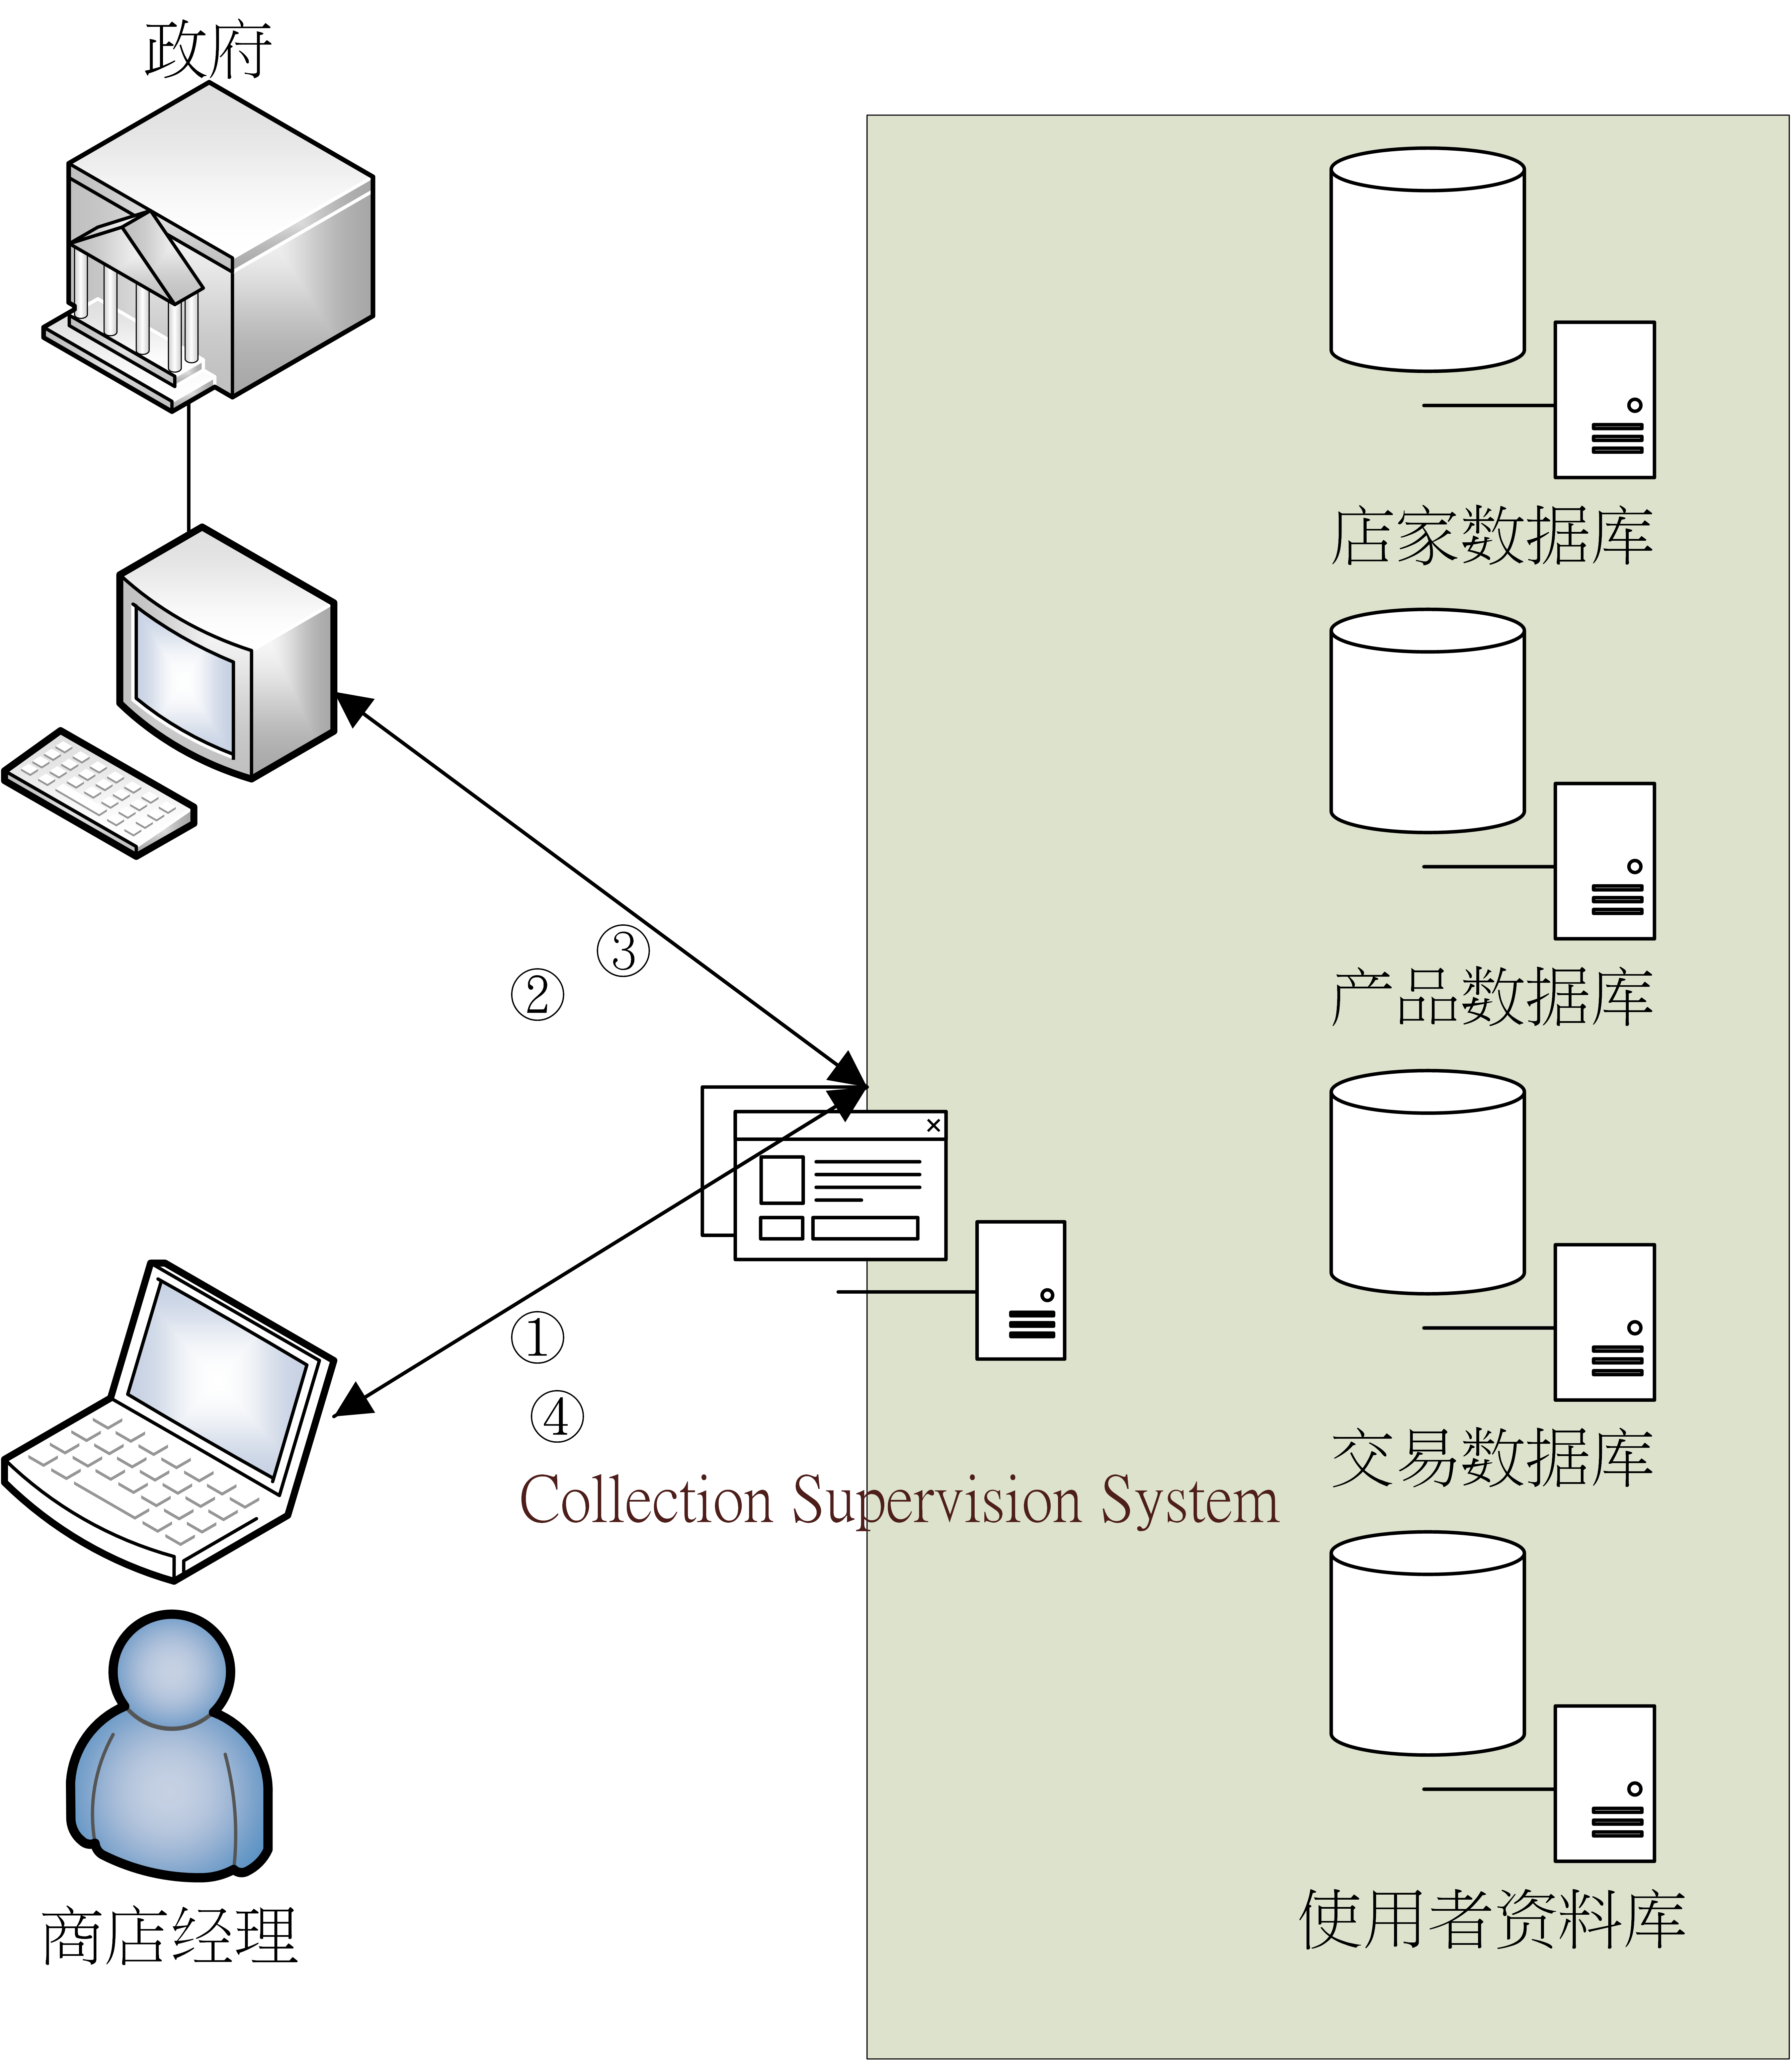
\includegraphics[width = 0.6\textwidth]{fig3.png}
		\caption{BRTMS和商家註冊流程的核心架構圖}\label{fig3}
	\end{figure}

	\begin{enumerate}
		\item 商戶必須在BRTMS註冊一個帳戶,並附有政府法規的商業證明。
		\item 區塊鏈的實名交易監督系統將自動向相應的政府金融監管機構提交商業申請,以審查該商店的加密貨幣交易業務。
		\item 如果政府批准商店的加密貨幣業務申請,服務器將激活商家在該收集監控系統中創建商店帳戶。
		\item 商家可以自由地登錄賬戶並添加商家想要出售的產品,並檢查他們的加密貨幣交易數據,例如產品庫存和產品交易記錄。
	\end{enumerate}

	\subsection{BRTMS架構與運作流程}
	具體的加密貨幣商家收銀金流監控系統運行過程如圖\ref{fig4}所示,我們以圖\ref{fig3}所設計出的系統架構進行擴增,首先我們需要與區塊鏈檢視器 (blockchain explorer)對接,而之所以該監控系統需要與區塊鏈檢視器對接是為了能夠最直接的比對交易被記錄的成交狀況,能夠達到即時性以及正確性,倘若擔憂單方面的依賴相信區塊鏈檢視器的成果,亦可以使用多家區塊鏈檢視器進行交叉參考,以避免因為一家公司的錯誤所帶來的影響。區塊鏈檢視器的目的是為了能夠快速地準確地比對該筆交易的成交,做為整筆交易提出到結算的環節之一。

	\begin{figure}[htbp]
		\centering
		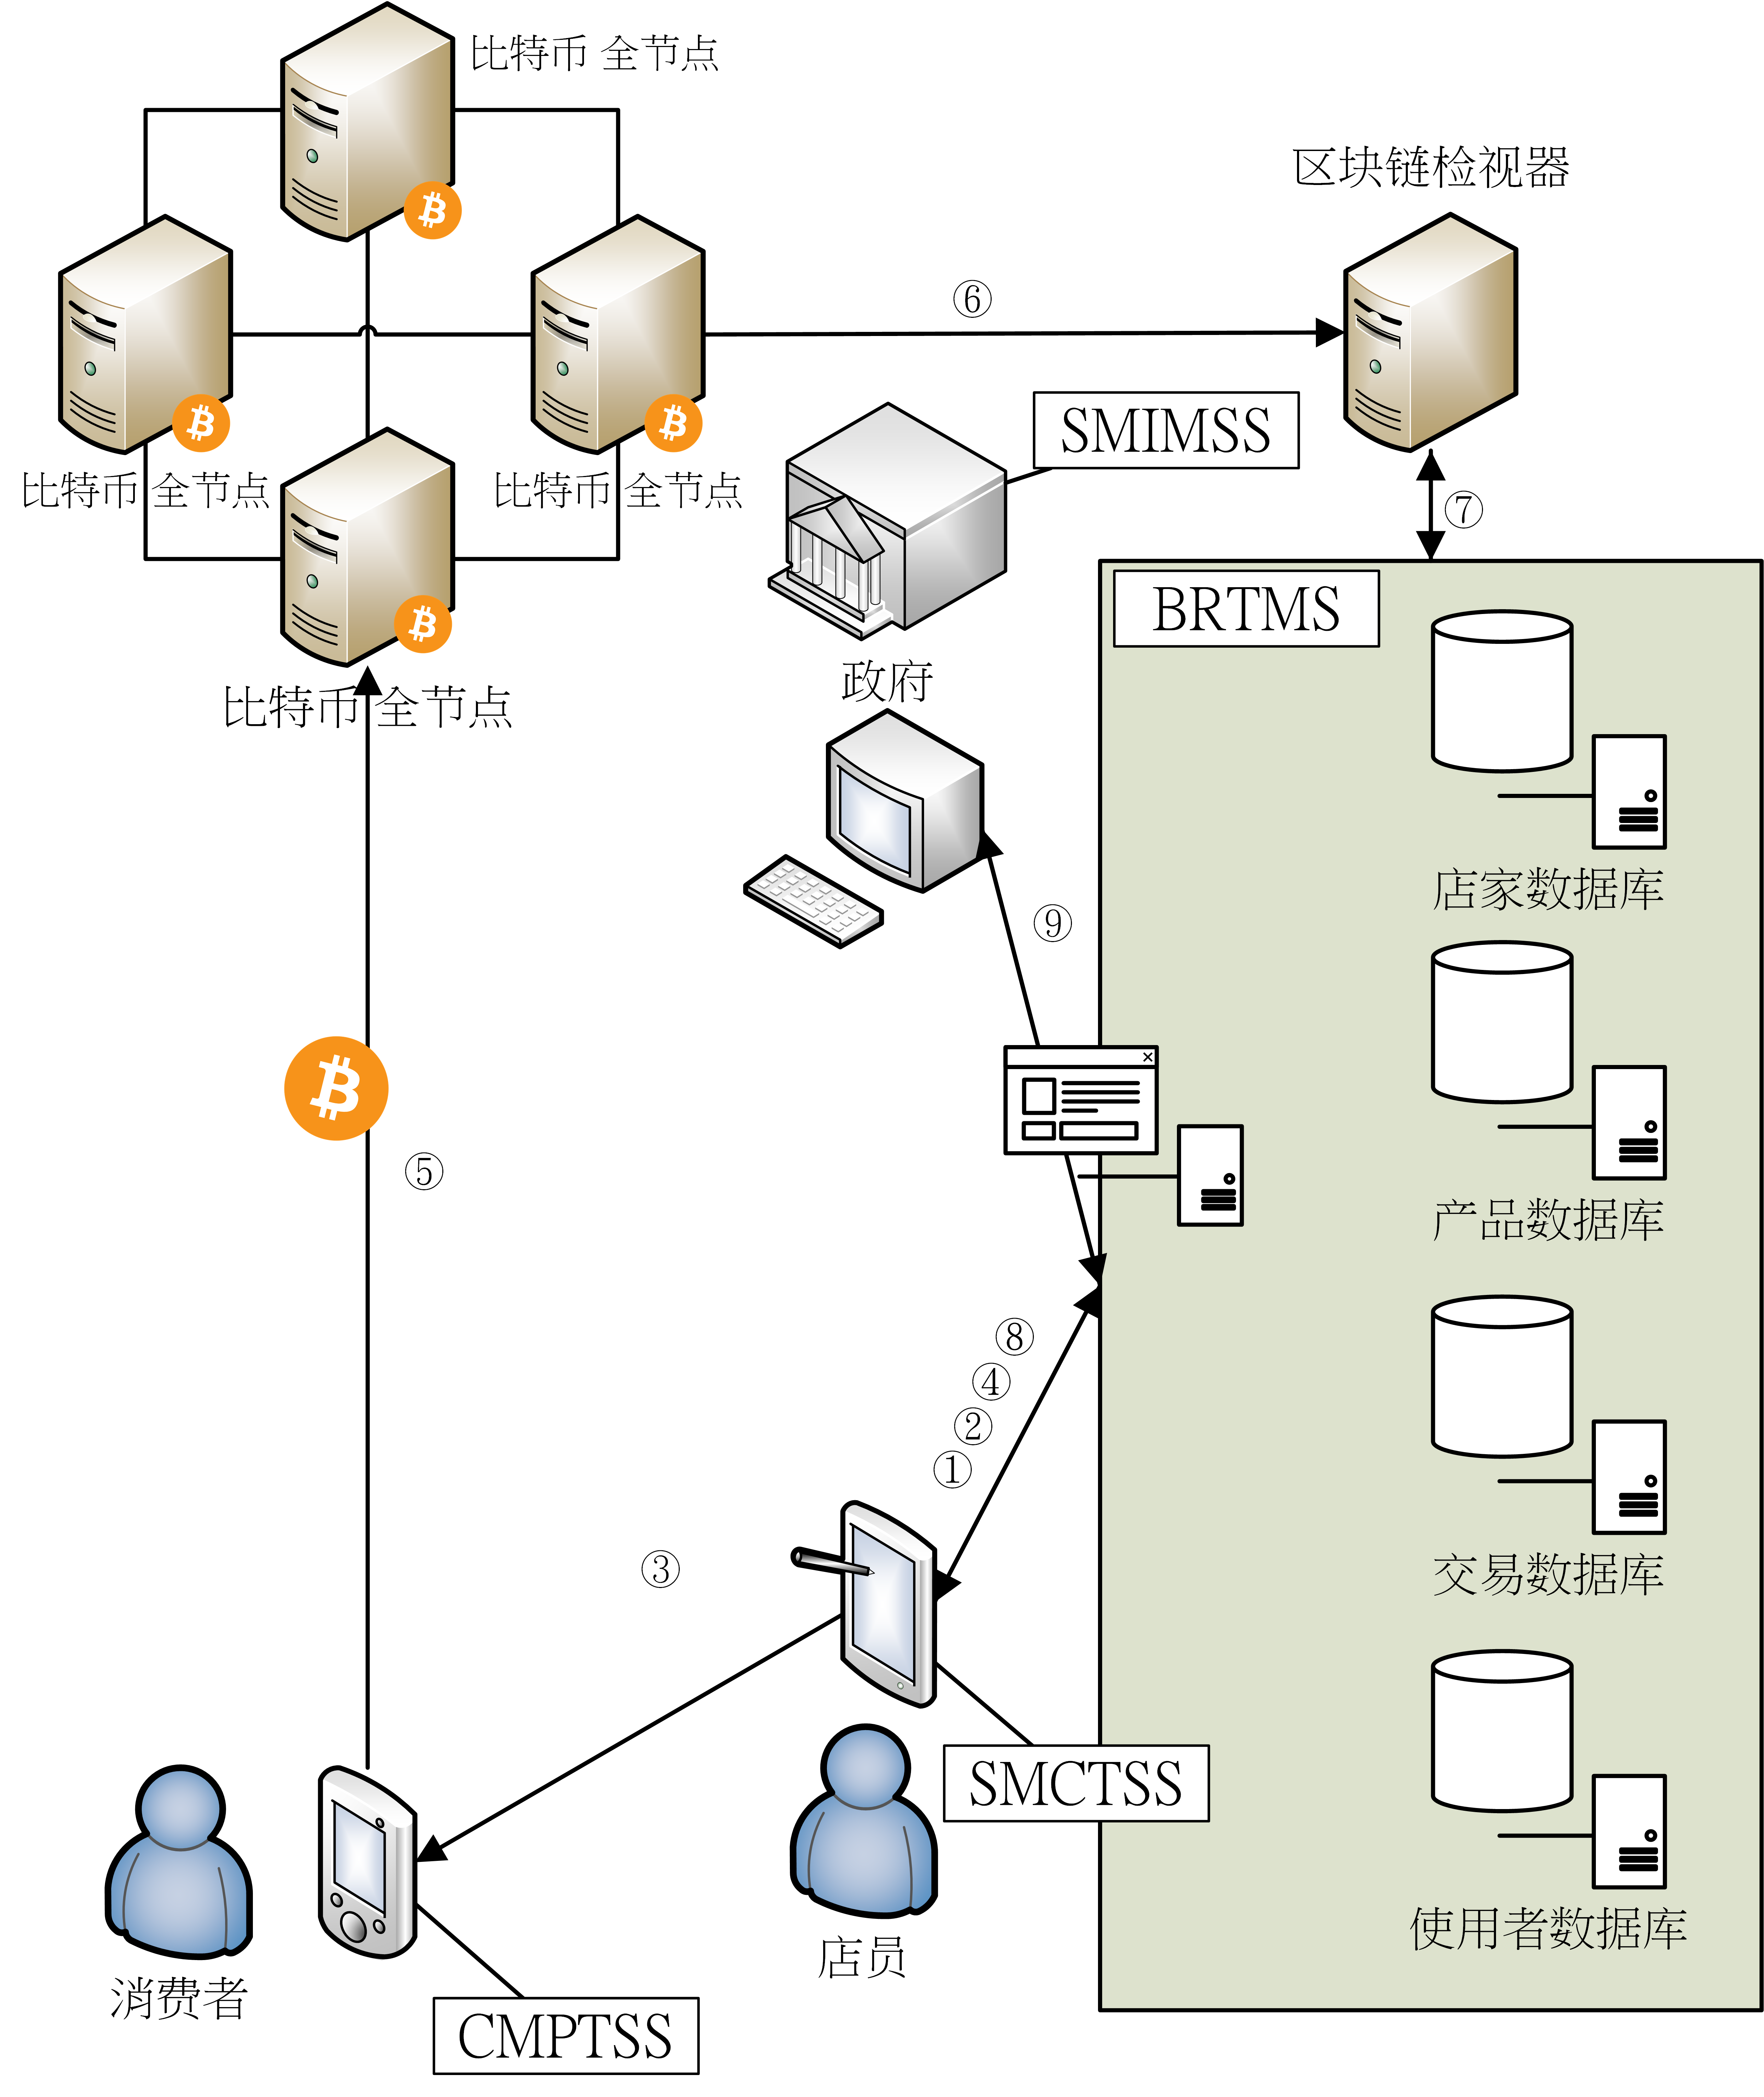
\includegraphics[width = 0.8\textwidth]{fig4.png}
		\caption{BRTMS的整體架構與功能示意圖}\label{fig4}
	\end{figure}

	圖\ref{fig4}區塊鏈的實名交易監督系統創建步驟描述如下:

		\begin{enumerate}
			\item 商家的店員將登錄到如圖\ref{fig3}所示的先前步驟創建的帳戶,以使用手持式平板電腦或智能手機訪問SMCTSS中的服務。如前所述,在能夠登錄到系統之前,商家帳戶必須由政府機構審計。
			\item 在成功登錄SMCTSS用於商戶加密貨幣流量監控系統時,移動設備將加載通過SMIMSS註冊的商店產品信息,然後創建產品目錄。商店的店員可以根據客戶的需求選擇所需的產品和數量。
			\item 店員使用設備完成客戶選定商品的產品信息後,移動設備上的NFC技術可用於將產品信息從附近店員的移動設備傳遞給消費者的移動設備,而無需物理交互。然後,消費者可以很容易地將自己的消費信息記錄成為發票等參考。在接收從商家店員設備向顧客設備購買產品消息的同時,顧客設備還將向商家的移動設備發送其自己的比特幣支付地址的消息。
			\item 商家的手持設備收到客戶確認購買所選產品的相應信息後,會將交易信息的副本發送給SMIMSS監控系統。消費者信息包括交易序列號、商戶ID號碼、商品號碼、購買的商品的數量以及加密貨幣的收款人地址以及消費者的支付地址。
			\item 收到消費者交易信息後,即完成此次的加密貨幣支付。同時,此次交易的加密貨幣將發佈到比特幣網絡中進行驗證和記錄。
			\item 區塊鏈瀏覽器將開始分析在比特幣網絡中緩存池的所有交易以及區塊鏈中記錄的交易。
			\item 擬議的交易監控系統BRTMS將向區塊鏈檢視器提出請求。這個請求數據不僅包括存儲在BRTMS中的交易副本之加密貨幣收款人地址(如圖\ref{fig3}的第4步所述),還包括客戶預期付款的加密貨幣支付地址。區塊鏈瀏覽器使用請求數據來檢查交易是否存儲在區塊鏈中,或者交易還在等待確認。如果交易已被確認並存儲在區塊鏈中,則交易數據庫中“交易確認”字段的值將更改為“1”,否則其默認值為"0"。
			\item 當“交易確認”字段中的值為“1”時,“交易已完成”消息可發送至商店平板電腦上運行的商店和商品信息管理子系統(SMCTSS)。
			\item 政府財政監督部門可以審查擬議BRTMS中的所有交易信息,以作為稅收審計參考。
		\end{enumerate}

\section{以多重簽章優化區塊鏈的實名交易監督系統之設計} 

在這樣的機制下,雖然Green Address 沒有減少交易確認時間,但是只要是用Green Address 即可確保雙重支付攻擊是不會發生的,對商家或是收款人而言,可以得到在即時交易中不被雙重支付攻擊的保障,提升未進入區塊鏈的交易可信度,進而創造出即時交易的可行性。 

本節將詳述本系統之商家註冊、Green Address錢包創建與驗證交易的運作流程與相關數據庫架構,如圖\ref{gabpcss}所示。

	\begin{figure}[htbp]
		\centering
		\includegraphics[width = 0.8\textwidth]{gabpcss.png}
		\caption{多重簽章優化後的BRTMS整體示意圖}\label{gabpcss}
	\end{figure}

	\begin{enumerate}
		\item 商家以通過政府機構的審查稽覈的帳戶登入該系統。
		\item 系統載入該店家註冊的商品信息,店員可以依照客戶的需求進行點單選取數量。
		\item 快速建立交易清單,並透過Green Address建立一個全新的比特幣收款地址,再以Android Beam的方式將交易信息輕鬆地傳達給消費者。
		\item 在商家店員的平板電腦收到這筆交易信息之後,會對本監督系統重送一個副本進行存檔。該交易信息包括由監督系統所提出的交易流水號、商家編號等信息。
		\item 消費者收到交易信息後,手機會自動開啟Green Address的付款頁面,確認金額無誤之後便能進行支付,此時便會以客戶的比特幣私鑰簽署交易,並等待Green Address機構節點的認證及發布。
		\item Green Address機構節點收到交易請求,並完成驗證非雙重支付攻擊後,以代理節點對應地址的私鑰簽署本次交易,並廣播至比特幣節點中。
		\item 區塊鏈檢視器便會開始分析網絡中所有存在緩存池中的交易,以及已經被記錄到區塊鏈中的交易。
		\item 本交易監督系統會向區塊鏈檢視器查找,檢查該筆交易是否已經存在於緩存池當中,若已經確認進入緩存池,則認定該筆交易成立並完成付款。
		\item 在交易確認之後,便向商家店員的平板電腦送出交易已經成交的信息,此時完成交易,於此同時也將該筆交易信息建置於系統數據庫內。
	\end{enumerate}